\chapter{Testbench}
\begin{figure}[h!]
	\centering
	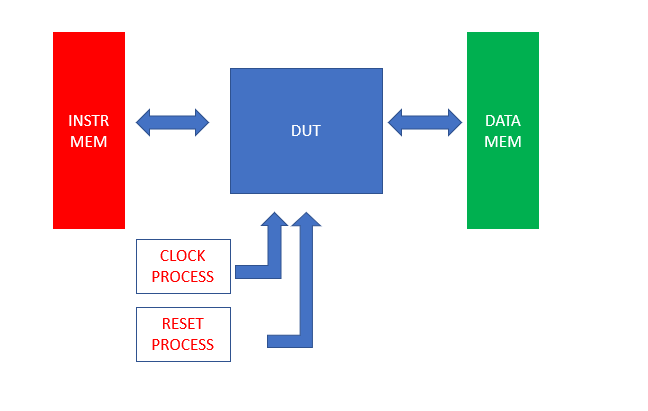
\includegraphics[width=10cm]{./images/Testbench}
	\caption{Testbench organization}
	\label{fig4.1}
\end{figure} 
The Clock process generates the clock signal for the entire processor and has a period of 20ns (for the testbench); in this way the processor is tested at 50MHz. \\
Our goal was to verify if the processor works correctly, without considering the performance, for this reason we have tested it at a low frequency.\\
The reset process initialize all the component. This signal is active for 15ns then it is disabled.\\
A good way to start the simulation is to reserve a clock cycle to reset the entire processor (without fetching any instruction in this phase). The signal that gives the reset will be active low for 15ns and then it will go up again (off) until the end of the simulation. After the reset phase, the first instruction in the instruction memory will be fetched and the processor will start to perform its tasks.

Before describing the content of the instruction memory in the vhd file, it was necessary to get some instructions in order to perform the test.
To achieve this, an assembly program was loaded in the RARS simulator, returning the instructions (reported in hexadecimal) that have to be written in the instruction memory (*).
After getting the list of all instructions, the instruction memory was filled, interleaving each instruction with three "empty lines" (x"00000000")  in such a way that the program counter update(PC+4) was respected.\\

The results are written in the Register file or in the Data memory, depending on which instruction is executed.

For what concerns the Instruction and Data memory we have implemented both like an array of 32 bits.\\
This because both memory are not so big, we have decided to implement them without resorting to a specific structure.\\

\begin{verbatim}
	*     in memory settings -> compact, Data at address 0 was selected
\end{verbatim}
\begin{figure}[h!]
	\centering
	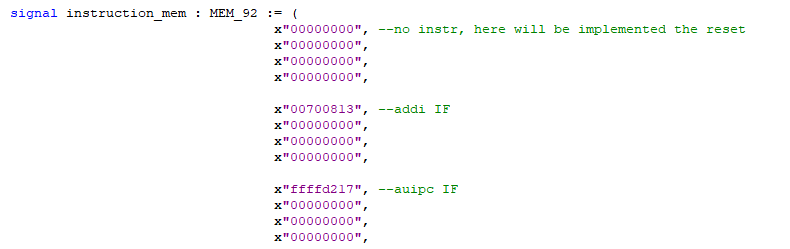
\includegraphics[width=18cm]{./images/Imem}
	\caption{Memory example}
	\label{fig4.2}
\end{figure} 

\newpage
\section{ABSV testbench}

We performed a separate testbench to test the ABSV instruction. We wrote as a first instruction the addi that adds a negative number (like "-7") to the content of register zero (that in this case is 0) and then it writes back the result to register sixteen. In this way we simply wrote the value "-7" in register sixteen.
After that the second instruction (ABSV) is performed and take the value of register sixteen and the ALU performs the absolute value operation storing it in register two. From the testbench it results that the new value is 7, therefor the instruction worked as intended.\\\\\\

\begin{figure}[h!]
	\centering
	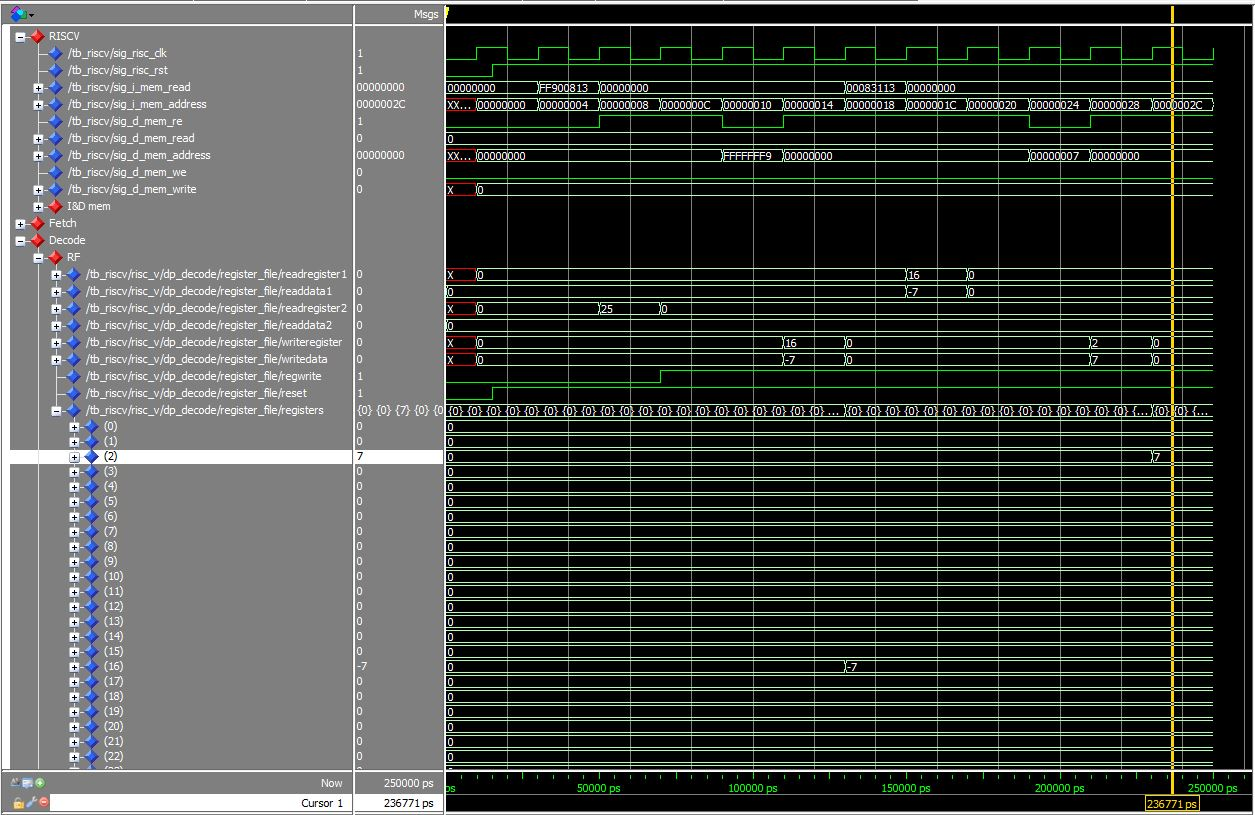
\includegraphics[width=18cm]{./images/TB_ABSV_waves}
	\caption{Memory example}
	\label{fig4.2}
\end{figure} 